
%==============================================================%
This user's manual is intended for first-time users
of the regional climate/weather forecasting model \scalerm.
The manual is based on
the meteorology/climate library {\scalelib} version \version.
The current version of \scalelib contains a regional model \scalerm
and a global model \scalegm.
%Only a dynamical core is provided for the latter.
This version of the user's manual explains how to use \scalerm in detail.
A description of \scalegm is planned for the next release.

The structure of this document is as follows:
Part \ref{part:overview} provides an overview of \scalelib,
Part \ref{part:install} describes how to install \scalerm
along with the system requirements. Using simple examples,
Chapters \ref{chap:tutorial_ideal} and \ref{chap:tutorial_real}
explain the basic use of \scalerm
using examples of an ideal experiment and an real atmospheric experiment, respectively.
Since these chapters are constructed as a series of tutorials, it is recommended that beginning users of \scalerm read these chapters meticulously.
Parts \ref{part:basic_usel} and \ref{part:advance_use}
describe how to change the model configuration and explain data format and available functions and tools.
Since each section is closed itself basically, these chapter can be utilized as a dictionary.


If you have any questions or comments, please contact us through the users’ mailing list\\ $\langle \verb|scale-users@ml.riken.jp|\rangle$.


\section{What is \scalelib?} \label{subsec:scale_feature}
%--------------------------------------------------------------%

Scalable Computing for Advanced Library and Environment, called {\scalelib}, is a software library that helps conduct research on climate and weather forecasting on any computer with ease. 
This library covers all processes related to such research: 
pre-processing, simulation, post-processing, and analysis. 
It has the following advantages:
\begin{itemize}
\item 
\scalelib is provided as an open-source software under the `` BSD-2 license''. It is free for use, modification, and redistribution, regardless of whether the user is a business or other enterprise.
\item 
\scalelib contains a regional model called the \scalerm ( SCALE-Regional Model ).
\item 
\scalelib prepares various schemes in a component, as outlined in the next section. They can be appropriately chosen according to the desired experiments of users.
\item 
\scalelib provides a framework for physical processes that can be called not only by \scalerm, but also by other numerical models.
\end{itemize}
For the details of the license, the interested reader can refer to the file \texttt{scale-\version/LICENSE} under the main directory. This explanation of its use is also provided on the SCALE webpage (http://scale.aics.riken.jp/). 

In this section, the concept of \scalelib and its relations to actual models are explained. It can be skipped, as it is not related directly to its practical use.

\clearpage
\Item{Relations between \scalelib library and models}

\begin{figure}[htb]
\begin{center}
  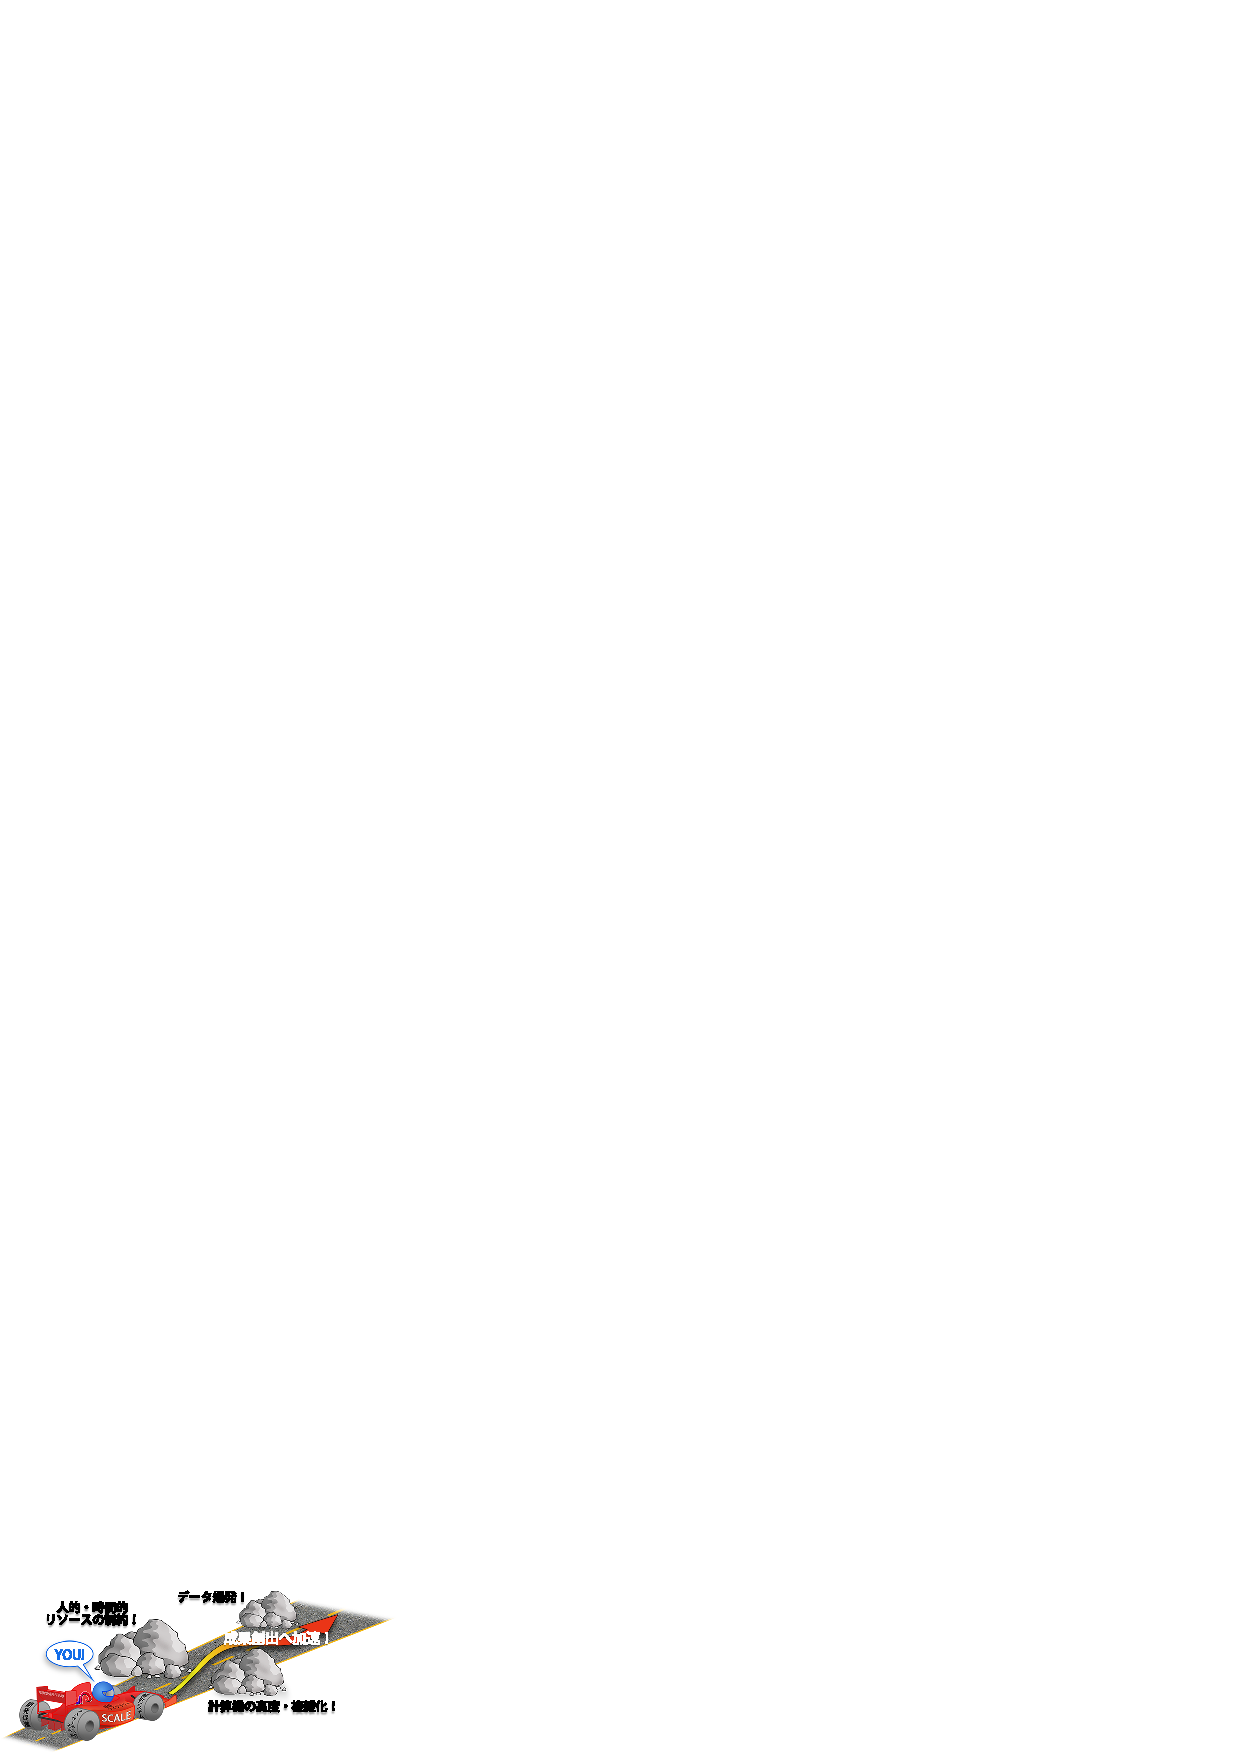
\includegraphics[width=0.9\hsize]{./figure/library.pdf}\\
  \caption{Aims of \scalelib}
  \label{fig:scale}
\end{center}
\end{figure}

\scalelib was developed in RIKEN with several outside contributors,
and its improvement and extension continue.
Figure \ref{fig:scale} shows the schematic concept of \scalelib.
As shown in this figure, SCALE aims to resolve various problems.
The development of \scalelib is considered in the context of its wide use
by devices ranging from small PC clusters to next-generation supercomputers.
For this purpose, scientists in meteorology/climate science
and computer science are cooperating.
%This has led to high computational performance of SCALE not only in supercomputers,
%such as the K Computer and the Fujitsu FX10,
%but also for general-purpose commercial computers,
%such as Intel processor-based machines.

\scalerm is a numerical model that fully uses \scalelib.
This model is contained in the \scalelib package,
as shown in Fig. \ref{fig:scale-rm}.
\scalelib manages the parallel processes,
file I/O, and inner-communication.
\scalelib also provides the solver for atmospheric flow ( dynamical core )
and physical processes such as micro-physics and radiation processes.
On the other hand,
\scalerm is constructed by combining functions provided by \scalelib.
\scalerm itself reads the input data of atmospheric status as prognostic variable,
and conducts time-integration.
Users can select a scheme in every component according to simulations they want.

\begin{figure}[hbt]
\begin{center}
  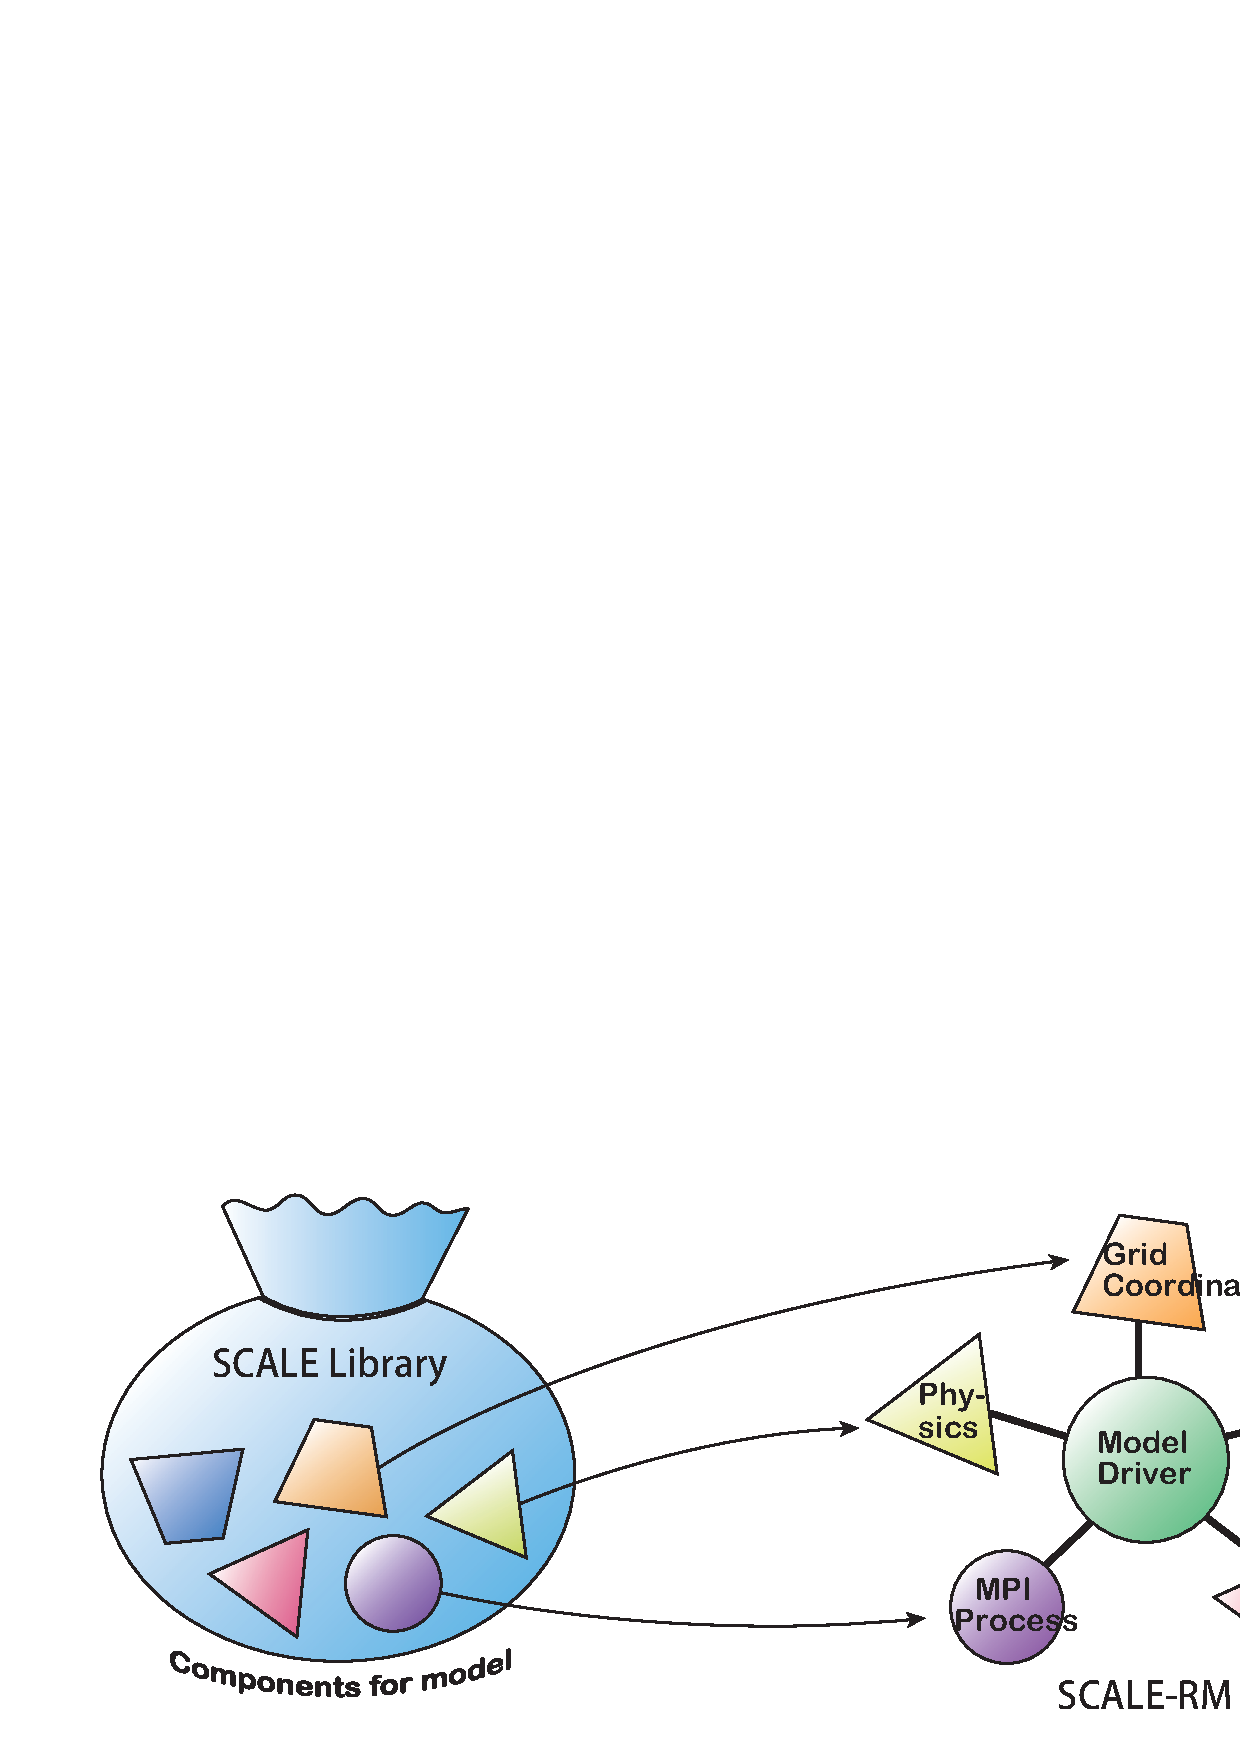
\includegraphics[width=0.9\hsize]{./figure/scale.pdf}\\
  \caption{Relationship between the library \scalelib and the model \scalerm}
  \label{fig:scale-rm}
\end{center}
\end{figure}


\section{Structure of \scalerm}  \label{subsec:sturcture_scale_rm}
%--------------------------------------------------------------%
All schemes in all components of \scalelib are available in \scalerm.
The components are categorized into three parts:
framework, dynamical core, and physical processes.
Components with various schemes already implemented
in the current version of \scalerm are listed below\footnote{Refer to \citet{scale_2015},\citet{satoy_2015b}, and \citet{nishizawa_2015} for the details of the model structure and the discretization method.}.

\subsubsection{Framework}
\begin{itemize}
 \item The three-dimensional (3D) Cartesian grid system based on actual distance
 \item 2D domain decomposition by Message Passing Interface (MPI) communication
 \item Several map projections commonly used
 \item Domain nesting system ( one-way, i.e., data transfer from parent domain to child domain. )
   \begin{itemize}
    \item  On-line nesting: concurrent execution of multiple domains).
    \item  Offline nesting: execution of computation in an inner domain after that in an outer domain.
   \end{itemize}
 \item Collective execution system of multiple cases, i.e., bulk job system
 \item \netcdf file I/O based on CF (Climate and Forecast) convention\footnote{\url{http://cfconventions.org/}}
   \begin{itemize}
   \item Selection of {\netcdf}3 and {\netcdf}4 formats
   \end{itemize}
 \item Generation of initial data for an ideal experiment
 \item Generation of topographical and land-use data, converted from external data
 \item Generation of initial and boundary data from external data
   \begin{itemize}
    \item 
      Supporting inputs from the WRF-ARW\footnote{\url{http://www.wrf-model.org/}} and
      \grads \footnote{\url{http://cola.gmu.edu/grads/}} formats.
   \end{itemize}
\end{itemize}

\subsubsection{Dynamical core}
\begin{itemize}
 \item Governing equations: 3D fully compressible non-hydrostatic equations
 \item Spatial discretization: finite volume method
    \begin{itemize}
      \item central advection schemes with 2nd-, 4th- and 6th-order accuracy
      \item upwind advection schemes with 3rd- and 5th-order accuracy
    \end{itemize}
 \item Time integration: selection from the ``fully explicit method'' 
   or the ``horizontally explicit and vertically implicit methods''
    \begin{itemize}
      \item \citet{Wicker_2002}'s 3 stage Runge--Kutta scheme with generally 2nd order accuracy
      \item Heun-type 3 stage Runge--Kutta scheme with 3rd order accuracy
      \item 4 stage Runge--Kutta scheme with 4th order accuracy
      \item 7 stage Runge--Kutta scheme with 6th order accuracy
    \end{itemize}
 \item Guarantee of non-negative value:
    \begin{itemize}
      \item Flux corrected transport method \citep{zalesak_1979}
      \item \citet{Koren_1993}'s filter: available only with the use of the 3rd-order upwind advection scheme
    \end{itemize}
 \item Numerical filter: hyper-viscosity and diffusion with 2nd, 4th, 6th and 8th-order differential operators 
 \item Topography: expressed using terrain-following coordinates
\end{itemize}


\subsubsection{Physical processes}
\begin{itemize}
\item Turbulence process: selectable from among the following
  \begin{itemize}
  \item \citet{smagorinsky_1963} \& \citet{lilly_1962}-type sub-grid scale turbulent model
    with the corrections by \citet{Brown_etal_1994} and \citet{Scotti_1993}
  \item \citet{Deardorff_1980} sub-grid scale turbulent model
  \item MYNN level 2.5 boundary scheme ( \citet{my_1982,nakanishi_2004} )
  \end{itemize}
\item Cloud microphysics: selectable from among the following
  \begin{itemize}
  \item 3-class 1 moment bulk scheme \citep{kessler_1969}
  \item 6-class 1 moment bulk scheme \citep{tomita_2008}
  \item 6-class 2 moment bulk scheme \citep{sn_2014}
  \item spectral bin scheme \citep{suzuki_etal_2010}
  \end{itemize}
\item Radiation process: a k-distribution-based broadband radiation transfer model ( \citet{sekiguchi_2008} )
\item Surface models
  \begin{itemize}
  \item Land model: heat diffusion/bucket model
  \item Ocean model: selectable from among the following
    \begin{itemize}
    \item fixed to initial condition
    \item input from external data
    \item slab model
    \end{itemize}
  \item Urban model: a single-layer canopy model \citep{kusaka_2001}
  \item Heat transfer coefficient at land and in ocean: selectable from among the following
    \begin{itemize}
    \item The bulk method using the universal function \citep{beljaars_1991,wilson_2001}
    \item Louis-type bulk method \citep{uno_1995}
    \end{itemize}
  \end{itemize}
\end{itemize}
